\documentclass[a4paper,12pt]{article}

\title{Math 31 \\ Limits and the Derivative}
\author{Jad Chehimi}

% document setup
\renewcommand{\familydefault}{\sfdefault}
\linespread{1.25}
\usepackage[margin=1.5in]{geometry}
\usepackage{setspace}
\usepackage{enumitem}
\usepackage{color,soul}
\setcounter{secnumdepth}{0}

% tools
\usepackage[hidelinks]{hyperref}
\usepackage{float}
%% images
\usepackage{graphicx}
\graphicspath{ {./images/} }
%% science
\usepackage{siunitx}
\usepackage{physics}

\begin{document}
\maketitle

% temp
\begin{center}
\Huge
Unfinished!
\normalsize
\end{center}
% temp

\tableofcontents

\pagebreak

\section{Factoring Brief Review}
\subsection{Differences of Square}
\Large
$x^2 - 4 = (x + 2)(x - 2)$
\normalsize

\subsection{Polynomial}
\Large
$2x^2 + 3x - 2$ \\
$\longrightarrow (2x^2 + 4x)(-x - 2)$ \\
$\longrightarrow \,\,2x(x+2) - 1(x+2)$ \\
$\longrightarrow (2x - 1)(x + 2)$
\normalsize

\subsection{Radical Fractions}
\begin{itemize}
    \item{
            Multiply everything by monomial denominator\\
            \Large
            $\frac{2}{\sqrt{2x}} \longrightarrow \frac{2\sqrt{2x}}{2x} \longrightarrow \frac{\sqrt{2x}}{x}$
            \normalsize
        }
    \item{
            Multiply everything by conjugate for polynomial denominators\\
            \Large
            $\frac{3}{2+\sqrt{x}} \times \frac{2-\sqrt{x}}{2-\sqrt{x}} = \frac{6-3\sqrt{x}}{4-2\sqrt{2} + 2\sqrt{x} - x} = \frac{6-3\sqrt{x}}{4-x}$
            \normalsize
        }
\end{itemize}

\subsection{Mixed Radicals}
\Large
$\sqrt{162} \longrightarrow \sqrt{9^2 \times 2} \longrightarrow \sqrt{9^2} \times \sqrt{2} \longrightarrow 9\sqrt{2}$
\normalsize

\subsection{Absolute Polynomial}
\Large
$|x-1| = 3$

$x-1 = 3$,
$x = 4$

$x-1 = -3$,
$x = -2$
\normalsize

\subsection{Adding/Subtracting Fractions}
Multiply both terms so that the denominators are the same, then add/subtract.\\
\Large
$\frac{2}{x-1} - \frac{3}{x+3}$\\
$\longrightarrow\frac{2(x+3)}{(x-1)(x+3)} - \frac{3(x-1)}{(x-1)(x+3)}$\\
$\longrightarrow\frac{(2x+6) - (3x-3)}{(x-1)(x+3)}$\\
$=\frac{-x+3}{(x-1)(x+3)}$
\normalsize

\subsection{Piecewise Functions}
Piecewise functions are functions with multiple inequalities/restrictions that dictate which function to use at specific $x$ values.

When graphing... 
\begin{itemize}
    \item{if an inequality is less/greater than a value, the plot point is \hl{not filled in}}
    \item{if an inequality is less/greater than \hl{OR equal to} a value, the plot point is \hl{filled in}}
    \item{if $x$ of different functions equal the same value, the graphs are continuous, and are filled in if one of the functions is inclusive}
\end{itemize}

If the inequalities do not state a function for a specific $x$ value (e.g. $x = 2$ for $2 < x < 2$) then that value \textbf{DNE}. (\hl{does not exist})

\subsection{Rational Function}
A function with a polynomial in the numerator and denominator.

\subsubsection{Vertical Asymptotes}
Zeros of the denominator of a rational function.

$x$ may approach these values, but never touch them.

\subsubsection{Point of Discontinuity}
Any vertical asymptote (zeros of denominator) \hl{before simplifying} a rational function.

These vertical asymptotes only applies to the unsimplified form; this makes it a point of discontinuity.

These points are gaps in a graph line, have no $y$ value, and therefore make a graph discontinuous.

\subsubsection{Horizontal Asymptotes}
Horizontal asymptotes describe the \hl{trend} of a function.

The graph line can cross over it fine, as opposed to vertical asymptotes.

\textbf{Determining Horizontal Asymptotes}
\begin{itemize}
    \item{degree of numerator $<$ degree of denominator\\$\longrightarrow y = 0$}
    \item{degree of numerator $=$ degree of denominator\\$\longrightarrow y = \frac{\textrm{leading coefficient of numerator}}{\textrm{leading coefficient of denominator}}$}
    \item{degree of numerator $>$ degree of denominator\\$\longrightarrow$ Divergent (no horizontal asymptote)}
\end{itemize}

\pagebreak

\section{Limits}
\Large
$$\lim\limits_{x \to a} f(x) = b$$
\normalsize
\begin{center}
The limit of $f(x)$ as $x$ approaches $a$ is $b$.
\end{center}

A limit is the value of $y$ as the $x$ approaches a specific value, as opposed to equaling a specific value. This is useful for points of discontinuity, where the exact value doesn't exist, but the value approaching does.

For instance, if the point of discontinuity of $f(x)$ is $x = -1$, then...
$$f(-1) = \textrm{DNE}$$
$$\lim\limits_{x \to -1} f(x) = -1$$

\subsection{Properties}
\begin{itemize}
    \item{$c = $ constant value \\ $\lim\limits_{x \to a} c = c$ \\ $\lim\limits_{x \to a} c f(x) = c \lim\limits_{x \to a} f(x)$}
    \item{$\lim\limits_{x \to a} [f(x)]^n = [\lim\limits_{x \to a} f(x)]^n$}
    \item{$\lim\limits_{x \to a} \sqrt[n]{f(x)} = \sqrt[n]{\lim\limits_{x \to a} f(x)}$}
    \item{The rest of the rules can be summarized as limits have distributive property. \\ e.g. $\lim\limits_{x \to a}[f(x) + g(x)] = \lim\limits_{x \to a} f(x) + \lim\limits_{x \to a} g(x)$}
\end{itemize}

\pagebreak

\subsection{Limits of Continuous Functions}
\subsubsection{Any Polynomial}
$y = f(x)$ is continuous at every value of $a$. 
$$\lim\limits_{x \to a} f(x) = f(a)$$
Just substitute $x$ in the function with $a$.

\subsubsection{Any Rational Function}
$y = \frac{f(x)}{g(x)}$ is continuous at every value of $a$ as long as $g(x) \neq 0$. (cannot divide by zero)
$$\lim\limits_{x \to a} \frac{f(x)}{g(x)} = \frac{f(a)}{g(a)},\; g(a) \neq 0$$
Just substitute $x$ in the function with $a$, unless $a$ makes the denominator equal to zero. If so, refer to the next section.

\subsubsection{Any Radical Function}
$y = \sqrt{f(x)}$ is continuous at every value of $a$ as long as $f(x) \geq 0$. (cannot root negatives)
$$\lim\limits_{x \to a} \sqrt{f(x)} = \sqrt{f(a)},\; f(a) \geq 0$$
Just substitute $x$ in the function with $a$, unless $a$ makes the function equal to a negative. If so, refer to the next section.

\subsection{Limits of Discontinuous Functions}
Identically to finding points of discontinuity, simplify/rationalize the function in a limit if it does illegal math (divide by zero, root negatives) until it doesn't.

$$\lim\limits_{x \to 4}(\frac{x^2 - 16}{x - 4})$$
$$\lim\limits_{x \to 4}(\frac{(x - 4)(x + 4)}{x - 4})$$
$$\lim\limits_{x \to 4}(x + 4) = 8$$

\section{One-sided Limits}
Limits of a function can be seperated into the value of approaching \hl{from the left} and \hl{from the right}. This is denoted with a superscript on $a$.
\begin{itemize}
    \item{From the left ($x < a$): \;\,\,$\lim\limits_{x \to a^-} f(x)$}
    \item{From the right ($x > a$): $\lim\limits_{x \to a^+} f(x)$}
\end{itemize}

This is only really relevant for graphs that end (such as $y = \sqrt{x}$, approaching from the side without a line is DNE) or piecewise functions.

\subsection{Continuous or Discontinous?}
\subsubsection{Continuous}
Continuous functions have a left approaching limit and a right approaching limit \hl{equal to one another}.

$$\textrm{if}\;\; \lim\limits_{x \to a^-} f(x) = \lim\limits_{x \to a^+} f(x)$$
$$\textrm{then}\;\; \lim\limits_{x \to a} f(x) = \lim\limits_{x \to a} f(a)$$

\subsubsection{Discontinuous}
Discontinuous functions have a left approaching limit and a right approaching limit \hl{not equal to one another}.

$$\textrm{if}\;\; \lim\limits_{x \to a^-} f(x) \neq \lim\limits_{x \to a^+} f(x)$$
$$\textrm{then}\;\; \lim\limits_{x \to a} f(x) = \textrm{DNE}$$

\pagebreak

\section{Limits to Infinity}
Limits of infinity either approach a value or DNE.

\subsection{Rules}
\begin{itemize}
    \item{
        Limits to infinity of normal numbers is often DNE.
        e.g.
        \begin{itemize}
            \item{$\lim\limits_{n\to\infty}{r^n} = \textrm{DNE}$ ($i\!f\!\!f \;|r| > 1$)}
            \item{$\lim\limits_{x\to\infty}{2^x} = \textrm{DNE}$}
            \item{$\lim\limits_{x\to\infty}{\frac{1}{x^{-3}}} = \textrm{DNE}$}
        \end{itemize}
    }
    \item{
        Limits to infinity of fractions with variable denominators is often infinity small, so 0.
        e.g.
        \begin{itemize}
            \item{$\lim\limits_{n\to\infty}{r^n} = 0$ ($i\!f\!\!f \;|r| < 1$)}
            \item{$\lim\limits_{n\to\infty}{\frac{1}{n}} = 0$}
        \end{itemize}
    }
    \item{The limit of infinity does not exist. \\$\lim\limits_{n\to\infty}{3^n} = DNE$}
    \item{$\lim\limits_{n\to\infty}{(-1)^n} = DNE$}
\end{itemize}

\subsection{Finding Limits to Infinity}
\begin{itemize}
    \item{Any fraction with a variable in the denominator will be zero. $$\lim\limits_{x\to\infty}{\frac{a}{x^b}} = 0$$}
    \item{Because of this, multiply a limit by something in order to put a variable under the terms, making them equal zero. e.g.}
\end{itemize}

$$\lim\limits_{x\to\infty}{\frac{6n+9}{3n-2}}$$
$$\frac{6n+9}{3n-2} \times \frac{\frac{1}{n}}{\frac{1}{n}}$$
$$\frac{6+\frac{9}{n}}{3-\frac{2}{n}} \longrightarrow \frac{6+0}{3-0}$$
$$\lim\limits_{x\to\infty}{\frac{6n+9}{3n-2}} = 2$$

\section{Derivatives}
The derivative of a function gives the slope of a tangent line that just touches the point $(x, f(x))$.

\subsection{Formulas}
\Large
$$f'(x) = y' = \frac{dy}{dx} = \lim\limits_{h\to0}{\frac{f(x+h)-f(x)}{h}}$$
\normalsize
\begin{figure}[H]
    \centering
    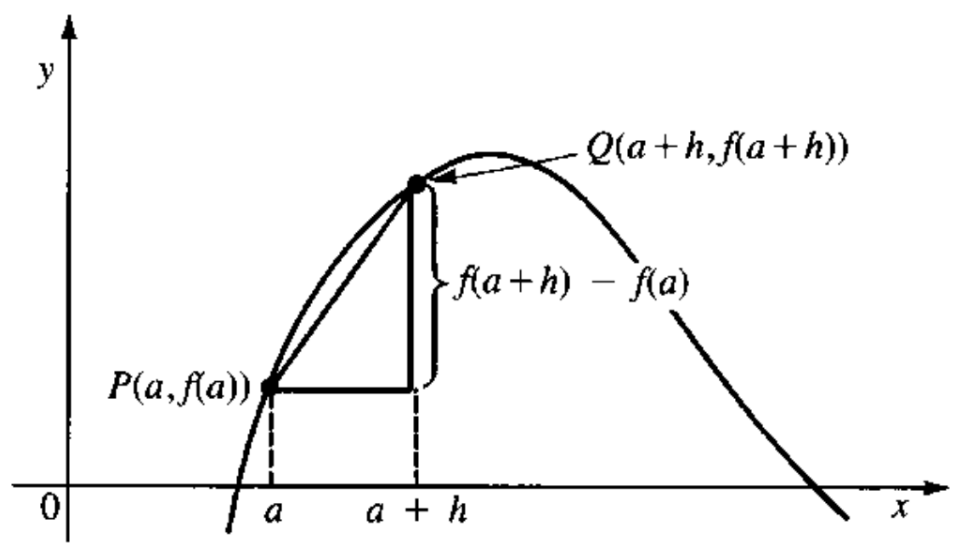
\includegraphics[width=\textwidth]{hgraph}
    \caption{The limits formula calculates the slope of a secant line (between two points on curve) and shrinks said line (by $h$ approaching zero) until it becomes a tangent line (the instantaneous slope of a point)}
\end{figure}

\subsection{Limits Method}
\subsubsection{Slope at Specific Point}
e.g. $f(x) = 3x^2 - 5x + 4$, find $f'(2)$
$$f(2) = 3(2)^2 - 5(2) + 4 = 6$$
$$\lim\limits_{h\to0}\frac{f(2+h)-f(2)}{h} \longrightarrow \lim\limits_{h\to0}\frac{[3(2+h)^2 - 5(2+h) + 4] - [6]}{h}$$
\begin{center}Expand and simplify until you are no longer dividing by zero.\end{center}
$$\lim\limits_{h\to0}{3h+7}$$
\begin{center}Calculate the limit: subsitute $h$ with $0$\end{center}
$$m = 7$$

\subsubsection{General Expression}
This is the actual derivative of a function. Inputting any value of $x$ into this expression is equivalent to the previous step.

e.g. $f(x) = 3x^2 - 5x + 4$, find $f'(x)$
$$\lim\limits_{h\to0}\frac{f(x+h)-f(x)}{h} \longrightarrow \lim\limits_{h\to0}\frac{[3(x+h)^2 - 5(x+h) + 4] - [3x^2 - 5x + 4]}{h}$$
\begin{center}Some tears and bloodshed later...\end{center}
$$f'(x) = 6x-5$$

For instance, the previous section can be solved using this function.
$$f'(2) = 6(2) - 5 = 7$$

\subsection{Slope to Equation}
To get an equation such as $y=mx+b$ from just a slope ($m$) and a given point $(x_1, y_1)$.

$$y - y_1 = m(x - x_1)$$

\subsection{Normal Line}
The "normal line" of a tangent is a line with a slope perpendicular to the tangent's slope.

Remember that the perpendicular slope of a slope is the negative reciprocal.

$$m = 12$$
$$\perp{m} = -\frac{1}{12}$$

\section{Differentiability}
\begin{itemize}
    \item{If $f'(x)$ exists, then $f(x)$ is \textbf{differentiable}}
    \item{If $f(x)$ is differentiable, then $f(x)$ is continuous at point $x$}
    \item{\hl{Continuity does not imply differentiability}}
\end{itemize}

\subsection{Non-differentiability Graphically}
A point on a graph that is often non-differentiable due to the limit of said point not existing. This usually occurs from the left and right limit not being equal.

These, graphically, could be...
\begin{itemize}
    \item{\textbf{Cusp}: sharp peak on a graph, like the tip of a triangle}
    \item{\textbf{Crossing Point}: gap between two graph lines}
    \item{\textbf{Vertical Asymptote}}
    \item{\textbf{Point of Discontinuity/Hollow Point}}
    \item{\textbf{Vertical Separation}: point that graphs switch in piecewise functions}
    \item{\textbf{End Point}: graph line ends at a point}
\end{itemize}

Other points that are non-differentiable could be...
\begin{itemize}
    \item{\textbf{Vertical Line}: slope/derivative is undefined}
\end{itemize}

\pagebreak

\section{Determine the Point Problem}
Recall this formula for calculating slope,
$$m = \frac{y_2 - y_1}{x_2 - x_1}$$

The derivative of a function calculates the slope of the tangent line touching point $x$ on said function. You can replace $m$ with the derivative then.

Replace the $x$'s and $y$'s with any given plot points. You can also give a point the coordinates of $(x, f(x))$ and solve.

These are example problems. You will likely be tested on questions similar to this.

\begin{figure}[H]
    \centering
    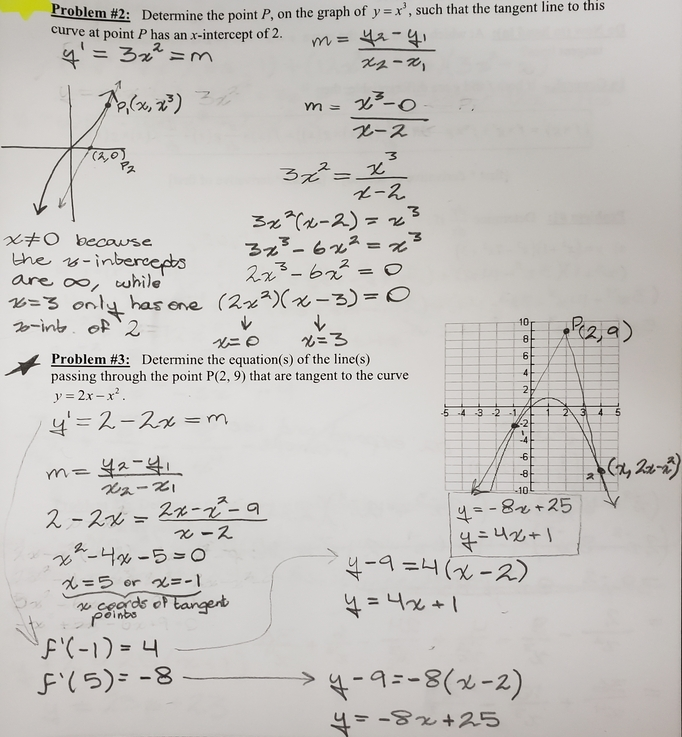
\includegraphics[width=\textwidth]{point}
\end{figure}

\section{Derivative Rules}

\subsection{The Power Rule}
\begin{center}
If $f(x) = x^n$, then $f'(x) = nx^{n-1}$
\end{center}
\begin{itemize}
    \item{Multiply pre-existing coefficients with $n$ \\ e.g. $8x^2 \longrightarrow 16x$}
    \item{Convert fractions and radicals into exponent form to apply the power rule \\ e.g. $\frac{4}{x^3} = 4x^{-3}$, $\sqrt{x^3} = x^{\frac{3}{2}}$}
    \item{The derivative of a variable with a \hl{degree of 1 equals 1} (since the power becomes zero) \\ e.g. $4x^1 \longrightarrow 4(1x^{1-1}) \longrightarrow 4$}
    \item{\hl{The derivative of a constant is zero}}
\end{itemize}

\subsection{The Sum and Difference Rule}
If both $f$ and $g$ are differentiable,
$$(f+g)' = f' + g'$$
$$(f-g)' = f' - g'$$
In other words, \hl{replace every term with its derivative}.

\subsection{The Product Rule}
If both $f$ and $g$ are differentiable,
$$(f \times g)' = f \times g' + f' \times g$$
In other words, (first)(derivative of second) $+$ (second)(derivative of first)

\subsection{The Quotient Rule}
If both $f$ and $g$ are differentiable,
$$\left( \frac{f}{g} \right)' = \frac{f' \times g - f \times g'}{g^2}$$

\subsection{With Respect To}
$$\dv{y}{x}$$
The derivative $\dv{y}{x}$ is said to be "the derivative of $y$ with respect to $x$."

Imagine it as actually being "the derivative of $x$ \hl{when inside of} $y$."

Or ask yourself, "\hl{inside of the function $y$}, what is the derivative of $x$?"

This only becomes relevant when there are more variables than $x$ and $y$, such as the chain rule below.

\subsection{Chain Rules}
\subsubsection{The Chain Rule}
If $y = f(u)$ and $u = g(x)$, then...
$$\dv{y}{x} = \left(\dv{y}{u}\right)\!\!\left(\dv{u}{x}\right)$$

e.g. Determine $\dv{y}{x}$ if $y = u^2 + u$ and $u = x^3$.
\begin{itemize}
    \item{$\dv{y}{x} = (\dv{y}{u})(\dv{u}{x})$}
    \item{$\dv{y}{x} = (2u + 1)(3x^2)$}
\end{itemize}

\subsubsection{The Power/Chain Rule}
The Power/Chain rule is the same as the Chain rule, but may be easier to understand.

If $y = u^n$ and $u = g(x)$, then...
$$\dv{y}{x} = nu^{n-1}\times\dv{u}{x}$$

In the simplest terms, treat the entire function as a variable and get the derivative of that. (imagine it as getting the derivative outside the brackets). 

Then, multiply that by the derivative of the function inside the brackets.

e.g. Determine $\dv{y}{x}$ of $y=(2x-7x^2+9)^{-2}$.
\begin{itemize}
    \item{Let $u = 2x-7x^2+9$}
    \item{$y = u^{-2}$}
    \item{$y = (nu^{n-1})(\dv{u}{x})$}
    \item{$\dv{y}{x} = (-2u^{-3})(2-14x)$}
\end{itemize}

\subsection{Product/Quotient and Chain Rules}
For some questions you may need to multiple rules when there are multiple "functions" with exponents.

\begin{itemize}
    \item{Use product/quotient rules between the two "functions"}
    \item{In those rules, you need to get derivatives of functions. Use chain rule in these scenarios}
    \item{After simplifying both sides of the $+$ or $-$, try to factor out anything}
    \item{The last thing you should try is expanding and adding like terms}
\end{itemize}

e.g. $f(x) = (x^2-1)^3(2-3x)^4$, what is $f'(x)$?
\begin{itemize}
    \item{$f'(x) = [(3(x^2 - 1)^2)(2x)](2-3x)^4 + [(4(2-3x)^3)(-3)](x^2-1)^3$ \\Inside the square brackets is chain rule, outside the square brackets is product rule}
    \item{$f'(x) = 6x(x^2-1)^2(2-3x)^4 + -12(x^2-1)^3(2-3x)^3$ \\Simplifying both sides of the +/-}
    \item{$f'(x) = 6(x^2-1)^2(2-3x)^3[x(2-3x) - 2(x^2-1)]$ \\Factoring out}
    \item{$f'(x) = 6(x^2-1)^2(2-3x)^3[2x-3x^2 - 2x^2+2]$ \\Expanded}
    \item{$f'(x) = 6(x^2-1)^2(2-3x)^3[-5x^2+2x+2]$ \\Add like terms}
\end{itemize}

\section{Implicit Differentation}
To get the derivative of equations where $y$ is in the equation. (rather than $y = f(x)$, its could be like $x + y = c$)

\begin{itemize}
    \item{Get the derivative of each term like normal, all aforementioned rules still apply}
    \item{Everytime you get the \hl{derivative of $y$, append $\dv{y}{x}$ (aka. $y'$)} to it}
    \item{
        \hl{Solve for $\dv{y}{x}$/$y'$}
        \begin{itemize}
            \item{Get any terms that include $y'$ to one side, and simplify/factor until the equation is $y' = ...$}
        \end{itemize}
    }
\end{itemize}

e.g. $x^2 + y^2 = 16$, what is $y'$?
$$2x + 2yy' = 0$$
$$y' = \frac{-2x}{2y} = \frac{-x}{y}$$

\section{Higher Order Derivatives}
The derivative of a derivative is denoted with increasing prime "ticks".
\begin{center}
    $f''(x) = f'(f'(x))$ (2nd derivative of $f(x)$)\\
    $f'''(x) = f'(f'(f'(x)))$ (3rd derivative of $f(x)$)\\
    $f^{(n)}(x)$ ($n$th derivative of $f(x)$)
\end{center}

e.g. 
\begin{itemize}
    \item{$f(x) = x^8$}
    \item{$f'(x) = 8x^7$}
    \item{$f''(x) = 56x^6$}
    \item{$f'''(x) = 336x^5$}
    \item{$f^{(5)}(x) = 6720x^3$}
\end{itemize}

\subsection{Involving Implicit Differentiation}
\begin{itemize}
    \item{Find $y'$ like before}
    \item{When finding $y''$, subsitute any instance of $y'$ with its actual value that you found}
    \item{When finding $y''$, replace any instance of the original function (if you find it) with the actual value you were given in the question}
\end{itemize}

e.g. If $x^4 + y^4 = 16$, what is $y''$?
\begin{itemize}
    \item{
        Get $y'$\\
        $4x^3 + 4y^3y' = 0$\\
        $y' = \frac{-4x^3}{4y^3} = \frac{-x^3}{y^3}$
    }
    \item{
            Get $y''$. Notice how you still have to append $y'$ to all $y$'s.\\
            $y'' = \frac{(y^3)(-3x^2) - (-x^3)(3y^2y')}{(y^3)^2}$\\
            $y'' = \frac{-3x^2y^3 + 3x^3y^2y'}{y^6}$
        }
    \item{
            Notice how theres $y'$, and we have it, so subsitute.\\
            $y'' = \frac{-3x^2y^3 + 3x^3y^2(\frac{-x^3}{y^3})}{y^6}$\\
            $y'' = \frac{-3x^2y^3 - 3x^6y^{-1}}{y^6}$
        }
    \item{
            When we factor out a value, we can see the original equation. Subsitute it with $16$, since we were given that.\\
            $y'' = \frac{-3x^2y^{-1}(y^4 + x^4)}{y^6}$\\
            $y'' = \frac{-3x^2y^{-1}(16)}{y^6}$
        }
    \item{
            Make sure you remember your exponent rules for these steps.\\
            $y'' = \frac{-48x^2}{y^7}$
        }
\end{itemize}

\pagebreak

\section{Applications}
\subsection{Terms}
\begin{itemize}
    \item{\textbf{Displacement} ($s$)\\position, direct line from start to current position}
    \item{\textbf{Average Velocity}\\Velocity over time. $v_{\textrm{avg}} = \frac{\Delta{s}}{\Delta{t}} = \frac{s_2 - s_1}{t_2 - t_1}$}
    \item{\textbf{Instantaneous Velocity}\\Velocity at a specific time. $v_\textrm{inst} = \lim\limits_{\Delta{t}\to0}{\frac{\Delta{s}}{\Delta{t}}}$}
\end{itemize}

\subsection{Velocity}
The derivative of an equation for displacement will make it for velocity.

If $s = f(t)$ was a displacement equation, then...
$$f'(t) = \dv{s}{t} = \frac{\Delta{s}}{\Delta{t}} = v$$

\subsection{Acceleration}
The 2nd derivative of an equation for displacement will make it for acceleration.

If $s = f(t)$ was a displacement equation, then...
$$f''(t) = \dv{v}{t} = \frac{\Delta{v}}{\Delta{t}} = a$$

\pagebreak

\section{Related Rates}
In related rates problems, you are given the rate of change of one thing, and you need to find the rate of change of another thing.

\begin{itemize}
    \item{Find a formula that includes both your known variable and unknown variable}
    \item{Get the derivative of said formula, appending "prime" variables just like implicit differentiation}
    \item{Subsitute any variables and rates of variables you have, calculate by any means necessary if you can find them}
\end{itemize}

\subsection{Tips}
\begin{itemize}
    \item{It helps a lot to draw diagrams of the scenario}
    \item{When given values, avoid subsituting them into the formula until you have got the derivative of it; otherwise you remove the ability to subsitute the 'prime' variables}
    \item{If any rate is decreasing, make sure the rate is negative}
\end{itemize}

\subsection{Simple Example}
\emph{The radius, $r$, of a circular disc is increasing at a rate of \SI{3}{\cm/\s}.\\Determine the rate that the area is increasing, $A$, when $r = \SI{4}{\cm}$.}

$A' = \dv{A}{t} = \textrm{?}$

$r' = \dv{r}{t} = \SI{3}{\cm/\s}$

Find a formula...

$A = \pi r^2$

Get the derivative...

$A' = 2\pi r r'$

We know $r = 4$, and $r' = 3$...

$A' = 2\pi (4) (3)$

$A' = \SI{24\pi}{\cm\squared/\s}$

\subsection{Cylinder Question}
\emph{A cylindrical vase has a height of \SI{35}{\cm} and a radius of \SI{12}{\cm}.\\It is being filled with water so that the depth is increasing at a rate of \SI{2}{\cm/\s}.\\Determine the rate at which the water is being poured in to the vase.}

$V' = \textrm{?}$

$h' = \SI{2}{\cm/\s}$

$r = \SI{12}{\cm}$

Volume formula...

$V = \pi r^2 \cdot h$

$V' = (\pi r^2)(1h^0h') + (2\pi r r')(h)$ (product law)

We don't have $r'$, but because $r$ doesn't seem to change, $r' = 0$...

$V' = \pi r^2h'$

We know $h' = 2$ and $r = 12$...

$V' = \pi(12)^2(2)$

$V' = 288\pi$

\subsection{Cone Question}
Due to the nature of a cone having both changing radius and depth, you would have to solve for more than one variable in the derivative. This is not possible.

Therefore, you must convert any equations such that there is only one variable to solve for. For cone questions, you can use \textbf{similar triangles}: the ratio of sides of two different but similar triangles are equal to one another.

This ratio can either be either tan of both triangles (opp/adj), or same sides between both triangles. Both will give you the same answer.

$$\frac{\textrm{opposite side of 1st triangle}}{\textrm{adjacent side of 1st triangle}} = \frac{\textrm{opposite side of 2nd triangle}}{\textrm{adjacent side of 2nd triangle}}$$
$$\frac{\textrm{opposite side of 1st triangle}}{\textrm{opposite side of 2nd triangle}} = \frac{\textrm{adjacent side of 1st triangle}}{\textrm{adjacent side of 2nd triangle}}$$

\begin{figure}[H]
    \centering
    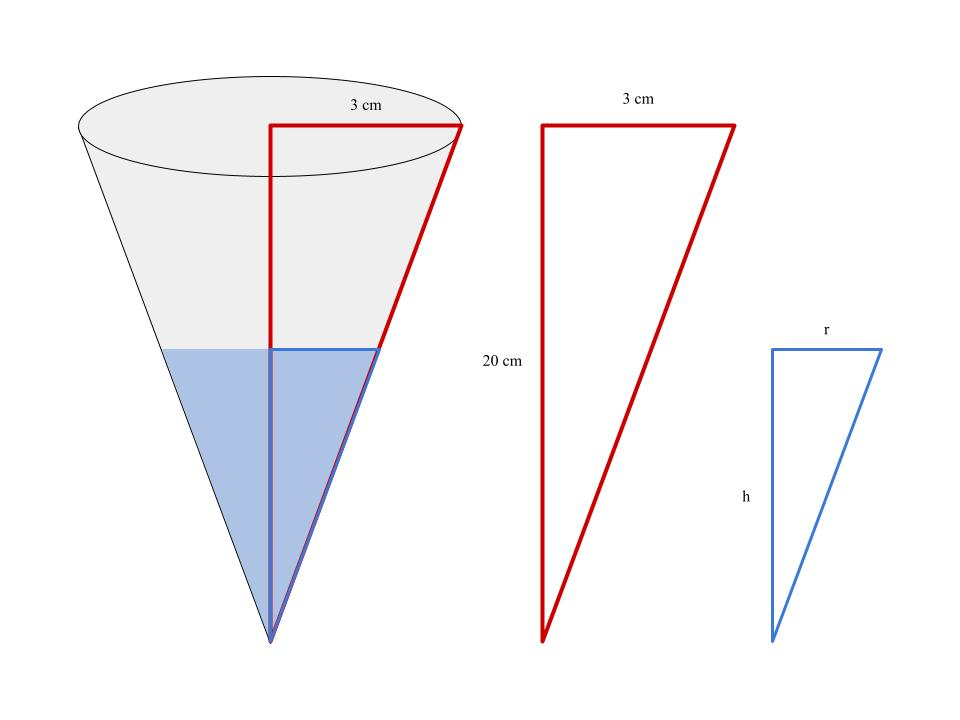
\includegraphics[width=\textwidth]{cone}
\end{figure}

\emph{A conical vase is being filled at a rate of \SI{10}{\cm\cubed/\s}.\\The vase is \SI{20}{\cm} high, and has a radius of \SI{3}{\cm} at the top.\\Determine the rate at which the water level is rising when the depth is \SI{10}{\cm}.}

The volume of a cone is...

$V = \frac{\pi}{3}r^2h$

The question only asks for $h'$, but we don't have $r$ \emph{or} $h$. Therefore, we got to convert $r$ into something that uses $h$.

Similar triangles allows us to do this. There are two triangles in this cone --- one for the whole space of the cone, and one for the space occupied by the water.

$\frac{r}{3} = \frac{h}{20}$, $r = \frac{3h}{20}$

Now we can rewrite the volume formula and continue as normal --- get the derivative and solve for $h'$.

$V = \frac{\pi}{3}(\frac{3h}{20})^2h$

$h' = \frac{40}{9\pi}$

\subsubsection{Missing Information}
If you are still missing information to fill in the formula, you can possibly get it with the similar triangles. For example, to get the radius of the water when the depth/height is 10.

$\frac{r}{3} = \frac{h}{20}$

$\frac{r}{3} = \frac{10}{20}$

$r = \frac{3}{2}$

The radius of the triangle of water in the cone is $\frac{3}{2}$ \hl{only when $h = 10$}. (instant value)

(While this gets us radius, it doesn't replace the process in the previous question, since you still don't know $r'$)

\pagebreak

\subsection{Object Filling Another Object}
\begin{itemize}
    \item{Find the rate of volume decreasing out of the first object (cone with a hole, or snowball melting)}
    \item{Flip the sign of this rate, and assign it to the object being filled up (like a box)}
    \item{Negative rate of volume leaving first object = Positive rate of volume entering second object}
\end{itemize}

\begin{figure}[H]
    \centering
    \includegraphics[width=0.95\textwidth]{fill}
\end{figure}

\pagebreak

\subsection{More Common Questions}
You should probably look at the booklet for good examples.
\begin{itemize}
    \item{\textbf{Sliding Ladder}: Nothing special, formula is pythagorem theorem, solve for the rate of change of a side}
    \item{\textbf{Distance Between Two Travelling Objects}: Pythagorem theorem, solve for the rate of change in the hypotenuse}
\end{itemize}

\subsection{Shadow Question}
Use similar triangles like before. Remember that the \hl{closer an object is to the light source}, the \hl{smaller the length of the shadow}.
\begin{figure}[H]
    \centering
    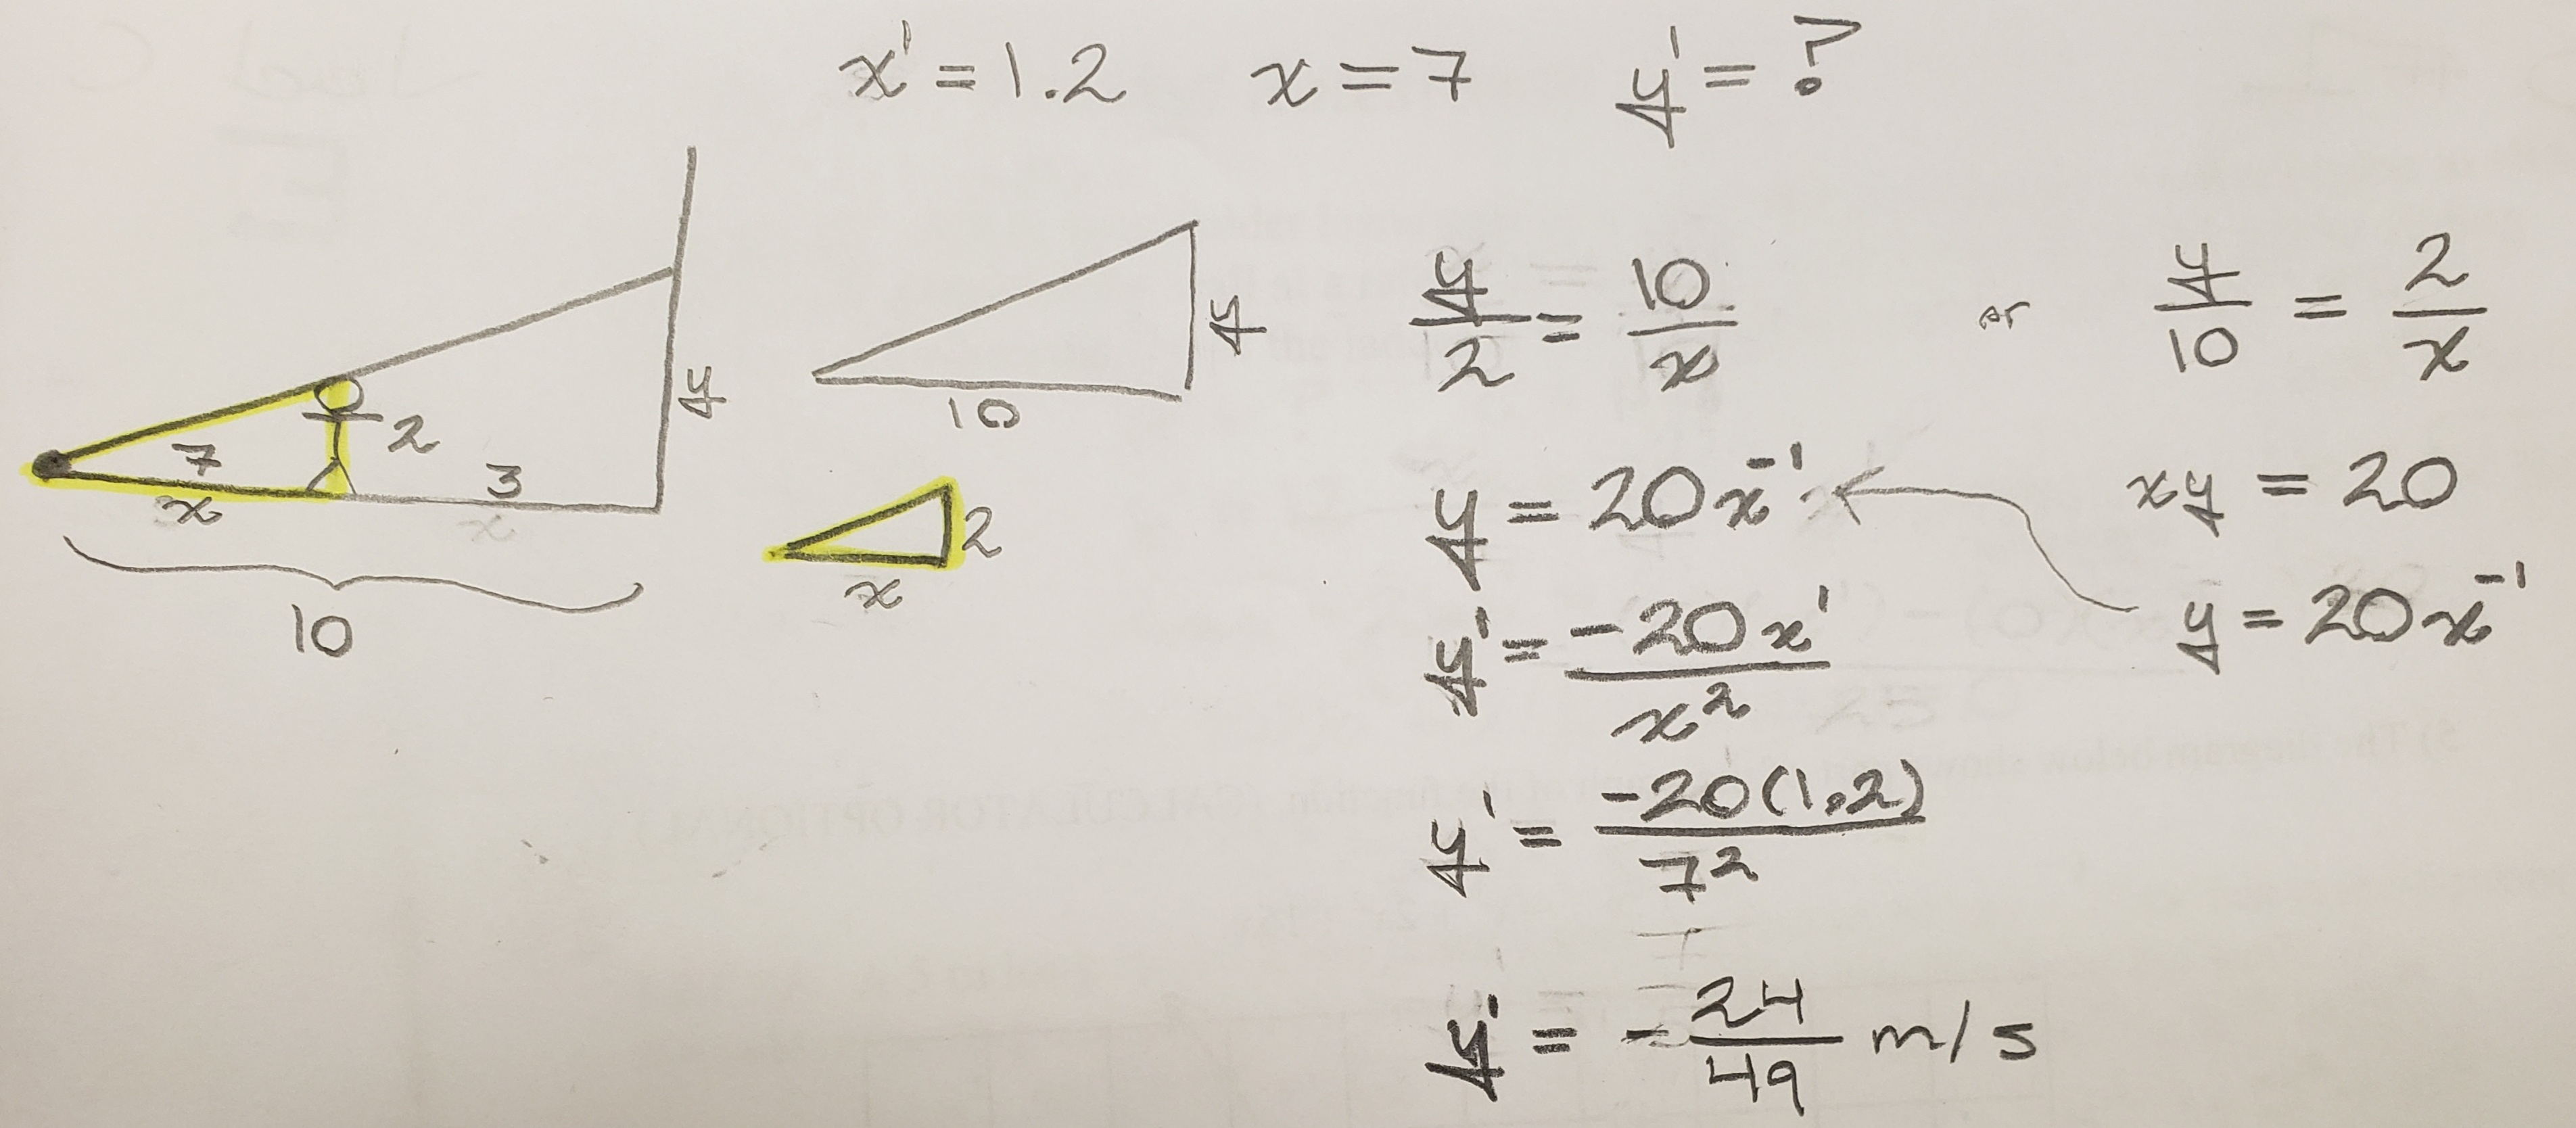
\includegraphics[width=\textwidth]{shadow}
\end{figure}

\subsubsection{Tips}
When choosing which variable to increase with the rate, make sure that variable is fixed and not affected by anything else, such as the person moving.

This is why, in the 2nd question for example, $x' = 2$ as opposed to $s' = -2$. $s$ has two points moving --- from the person to the end of the triangle --- as opposed to $x$ which only has one point moving --- from the stationary lamppost to the person.

\begin{figure}[H]
    \centering
    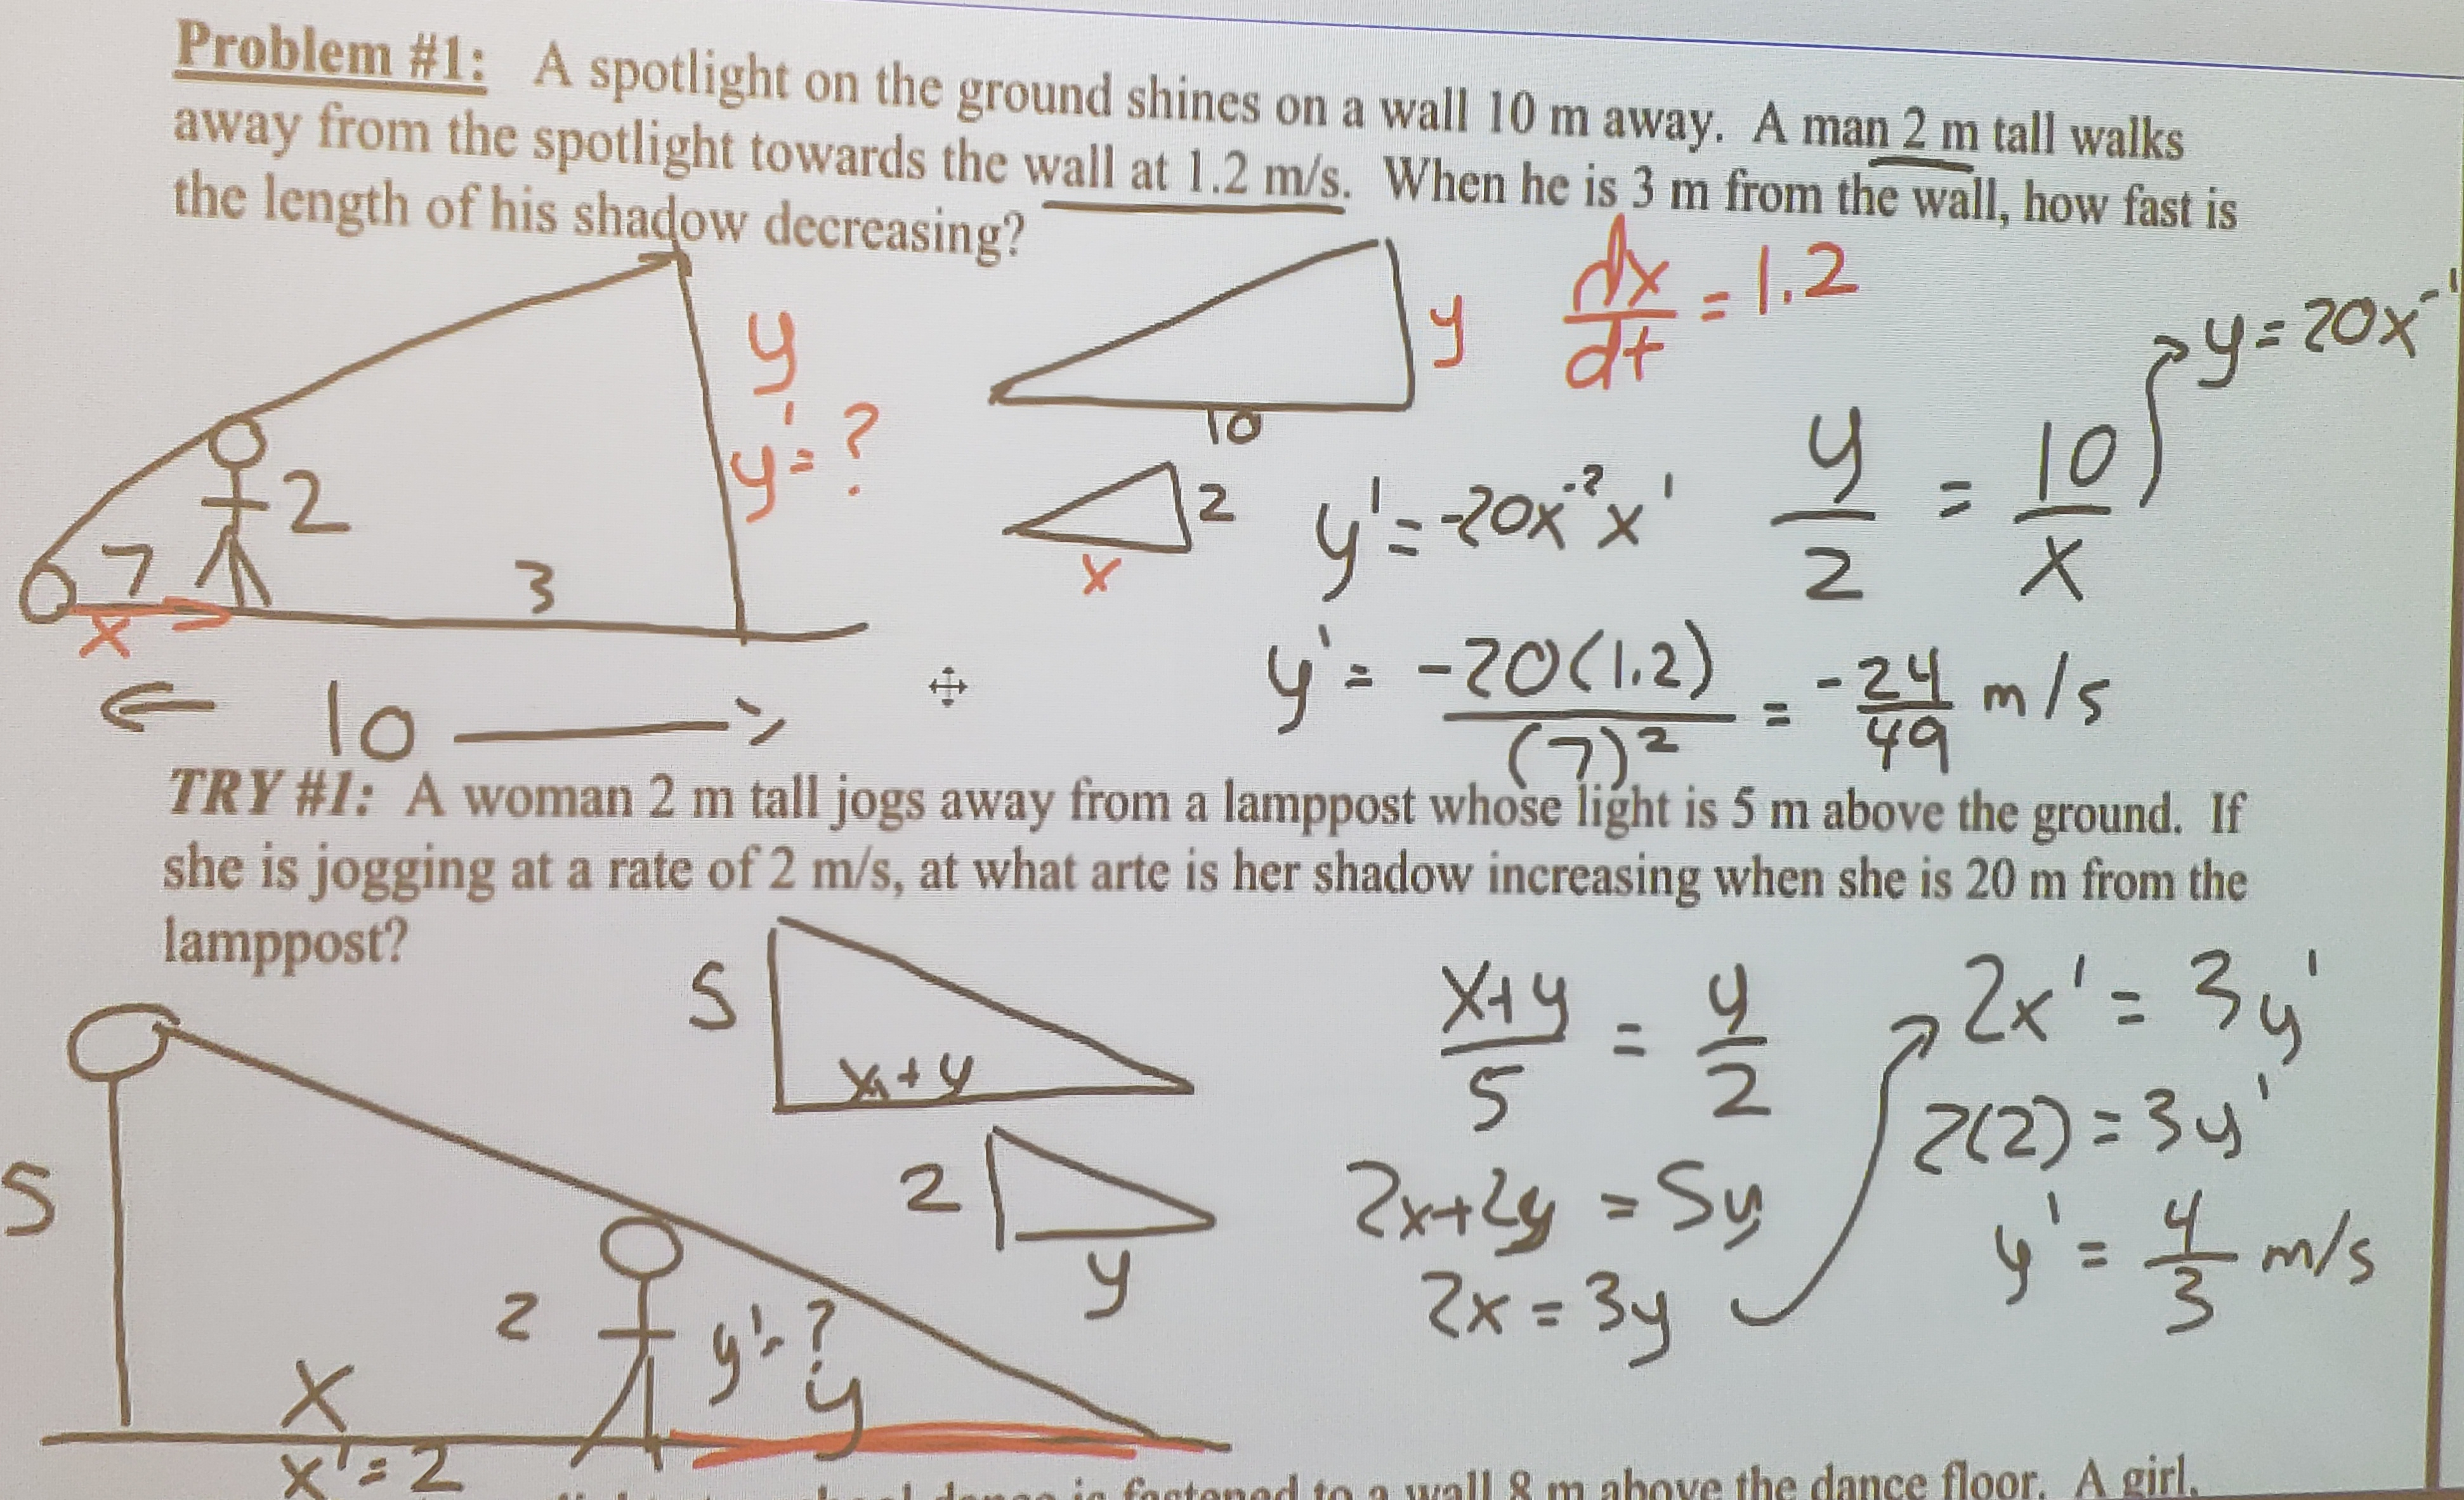
\includegraphics[width=\textwidth]{shadow2}
\end{figure}
\begin{figure}[H]
    \centering
    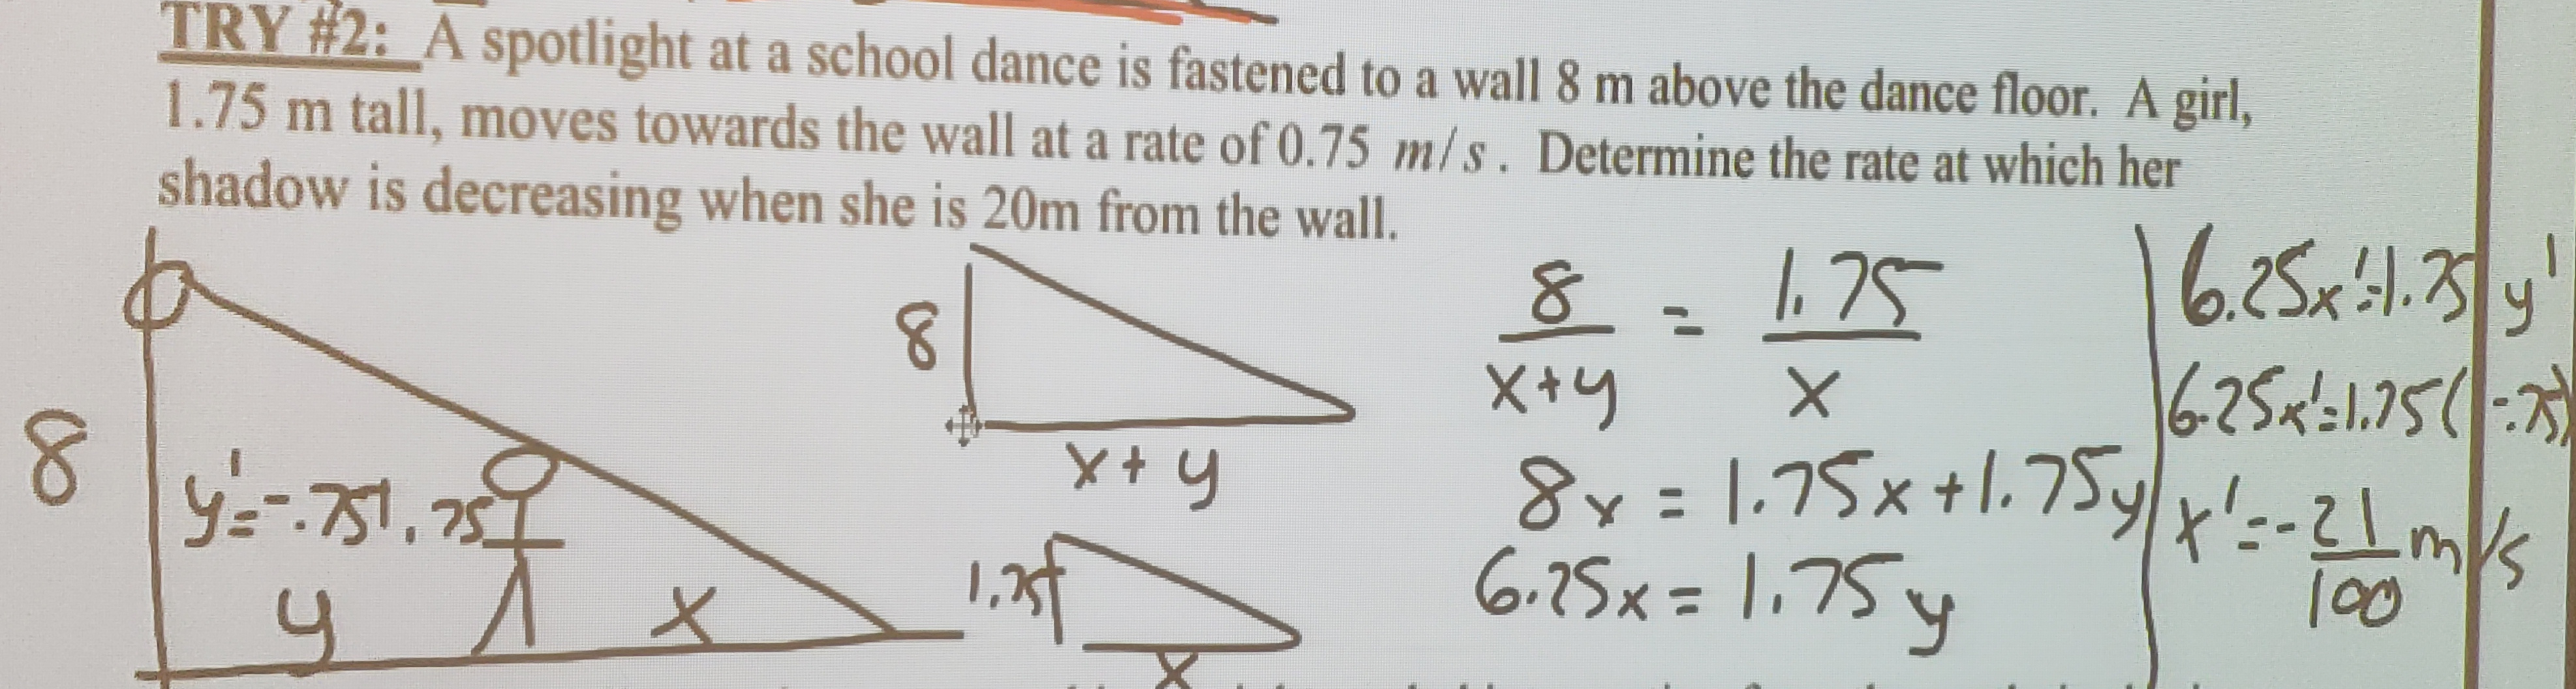
\includegraphics[width=\textwidth]{shadow3}
\end{figure}

\end{document}
